\begin{tikzpicture}
  \node[inner sep=0pt] (two-d) at (-6,3)
  {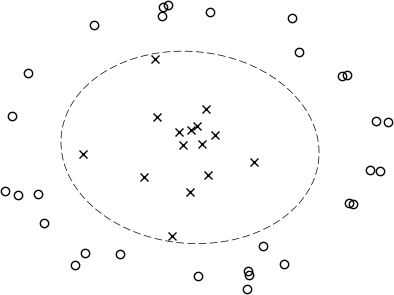
\includegraphics[width=.5\textwidth]{figure_3_3_2.png}};

  \node[inner sep=0pt] (three-d) at (-2,0)
  {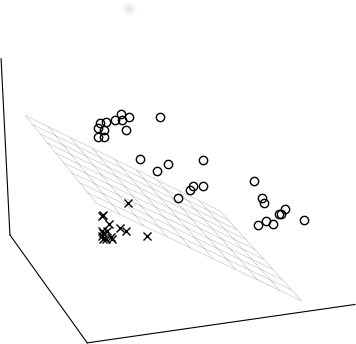
\includegraphics[width=.55\textwidth]{figure_3_2.png}};

  \draw[bend right,->]  (-7,1.6) to node [left] {$(1)$} (three-d);
  \draw[bend right,->] (-3.5,0.8) to node [right] {$(2)$} (-4.7,2.3);
    
\end{tikzpicture}

%%% Local Variables:
%%% mode: latex
%%% TeX-master: "learning_with_kernels"
%%% End:
